\documentclass{../../text-style}

\texttitle{Введение в Linux}

\begin{document}

\maketitle
\thispagestyle{empty}

\section{Что такое Linux}

Linux --- это семейство Unix-подобных операционных систем, объединённых более-менее общим ядром, набором стандартов и соглашений.
Ядро Linux имеет открытый исходный код, лежит в репозиториях, поддерживаемых сообществом, но имеет зеркало на GitHub (\url{https://github.com/torvalds/linux} (дата обращения: 24.02.2024)).
Вообще, Linux строится вокруг идеи свободного программного обеспечения (хотя Linux, Free Software Foundation и GNU --- это разные вещи, их не надо путать), поэтому сообщество очень щепетильно относится к защите от vendor lock-in, поэтому на GitHub и подобные хостинги целиком никогда не переедет.

Linux имеет огромное сообщество разработчиков, управляемых по иерархической структуре, в корне которой находится Линус Торвальдс --- собственно, первый разработчик ядра, который начинал писать Linux как студенческую работу на основе идей учебной ОС Minix от Эндрю Танненбаума (который сам по себе очень известный товарищ).
Открытость и вовлечённость кучи людей в процесс имеет свои плюсы и свои минусы:

\begin{itemize}
    \item всё, о чём вы можете подумать, скорее всего, кто-то уже сделал;
    \item пользователи имеют доступ к исходному коду, замечают проблемы, предлагают правки, поэтому популярное ПО (тем более --- ядро), скорее всего, очень стабильно и \enquote{вылизано} до блеска;
    \item никто никому ничего не должен, поэтому не очень популярное ПО может быть откровенно плохим;
    \begin{itemize}
        \item более того, часто разрабатывается красноглазыми школьниками, которые без идей, как программировать, но попасть в какой-нибудь дистрибутив Linux для них мечта --- в ядро их код не берут, но прикладные программы вполне.
    \end{itemize}
    \item нет единых стандартов, архитектуры, процесса, не только для прикладного ПО, но и для важных частей ОС.
\end{itemize}

Применяется Linux сейчас в основном как серверная ОС, и в этом плане она с большим отрывом лидирует (разве что другие UNIX-подобные системы типа FreeBSD, которые неопытный пользователь никогда не отличит от Linux, могут составить ей конкуренцию).
Также Linux, в силу открытости и модульности, применяется для встроенных устройств и разного специализированного оборудования, где нет требований реального времени%
\footnote{Системы жёсткого реального времени должны давать гарантию, что такая-то процедура будет выполнена за такое-то физическое время, например, за 20 миллисекунд. Linux не может давать такой гарантии.}.
Linux также несколько удобнее для профессиональной разработки, особенно для низкоуровневого программирования, под него более зрелый и удобный инструментарий.
Однако и Enterprise-, и веб-, облачная и т.п. разработка тоже часто ведётся на Linux, отчасти потому, что это достаточно удобно, отчасти чтобы быть ближе к окружению, в котором разработанная система будет работать.

Почему не весь мир работает на Linux --- у Linux не очень хороши дела для поддержки конечных пользователей.
Современные дистрибутивы очень дружелюбны (в былые времена иногда приходилось программировать на Си для повседневного пользования компьютером, что не очень), но гораздо хуже обстоят дела с поддержкой аппаратного обеспечения и с играми.
С аппаратным обеспечением дела обычно поправимы --- если производитель не выпускает официально ПО для Linux, это делают энтузиасты, и если что-то не заработало сразу, можно некоторое время пострадать (возможно, попрограммировав на Си), и заработает (в отличие от Windows, где, как правило, если что-то не работает, то всё).
Из того, с чем наверняка придётся столкнуться --- некоторая ненадёжность автоматической настройки дисплеев, так что заставить линуксовый ноутбук правильно выводить на проектор может быть неким вызовом (программировать не придётся, но копаться в конфигах в трёх разных местах --- возможно).
Заставить работать три монитора с разным разрешением от двух видеокарт разных вендоров так, чтобы выполнялось адекватное масштабирование пользовательского интерфейса --- автору так и не удалось.

С играми похуже, сообщество не считает их чем-то полезным, и там часто используются специфичные для Windows технологии, такие как DirectX.
Однако в последнее время игровые движки делаются кроссплатформенными, так что игры на них под Linux в целом работают, хотя иногда странно.
Но есть довольно много игр, которые не работают, и, видимо, никогда не будут.

Linux распространяется в виде дистрибутивов.
Само ядро не имеет никакого пользовательского интерфейса, даже консольного, и его можно понимать как скомпилированную библиотеку, которая всем управляет и предоставляет программный интерфейс для прикладных программ и системных утилит.
Ядро модульное, есть штуки, которые так и называются --- \enquote{модули}, их можно воспринимать как динамически загружаемые библиотеки, которые можно подгружать и выгружать прямо в процессе работы системы, и они обычно нужны для поддержки того или иного оборудования.
Однако чтобы пользователю работать с системой, нужна куча прикладных программ --- во-первых, шелл (shell), интерфейс командной строки, во-вторых, утилиты типа копирования файлов, в-третьих, графическая оболочка, в-четвёртых, пакетный менеджер, отвечающий за установку, обновление и удаление прикладных программ.
Всё это вместе, плюс начальная конфигурация системы, плюс политика обновления ПО и т.п. --- это и есть дистрибутив, то есть готовая к использованию система, которую можно поставить к себе на компьютер и начать ей пользоваться.
Дистрибутивов сотни, даже известных и широкораспространённых десятки.
Есть три-четыре популярных российских, которые на волне импортозамещения и ухода Microsoft стремительно занимают освободившуюся нишу в корпоративной и государственной сферах, и заодно и у обычных пользователей, хотя им приходится отчаянно конкурировать с западными.
Для корпоративных нужд требуется техподдержка, что с западными дистрибутивами может быть трудно, для домашнего использования техподдержка не нужна, поэтому вполне разумный выбор (хотя ходят слухи, что некоторые программы могут потихоньку гадить пользователям из России).

\subsection{Чем Linux хорош для программистов}

Linux популярен в программистском сообществе по целому ряду причин.
Наверное, основная --- бесплатность.
Linux можно ставить на виртуальные машины в каких угодно количествах, не платя за лицензию, а поскольку сейчас повсеместно используется виртуализация и контейнеризация, это может быть критично.
В правильно настроенном сервере \emph{каждый} делающий полезную работу процесс работает в собственном контейнере (или на целой виртуальной машине), так что на лицензиях на Windows и ПО для него даже крупная компания могла легко разориться.
Однако, как обычно, есть нюанс --- бывают и даже вполне распространены платные дистрибутивы.
Бесплатность открытого ПО вовсе не значит, что на нём нельзя зарабатывать --- покупая платный дистрибутив, пользователь покупает отсутствие проблем и техподдержку, если проблемы всё-таки возникнут, плюс, иногда, проприетарные специальные программы и сервисы, которых нет в открытом доступе.
Например, Астра Линукс распространяется именно по такой модели --- есть очень устаревшая бесплатная версия и свежая платная для корпоративных клиентов, с \enquote{правильными} гарантиями безопасности, включая гарантию защиты от \enquote{protestware}%
\footnote{\enquote{Protestware} --- программное обеспечение, которое, помимо полезных функций, пытается донести до пользователя позицию автора по какому-либо политическому или социальному вопросу, вплоть до попытки форматирования диска пользователей, которых автор считает в чём-либо виновными. В мире открытых систем огромной сложности весьма опасно (поскольку может быть \enquote{притянуто} зависимостями), и зачастую крайне неэтично. Не делайте так, какими бы благими ни были ваши намерения.}.

Вторая причина --- конфигурируемость.
Есть готовые дистрибутивы, включающие в себя всё, необходимое для работы.
Есть миниатюрные системы, которые, кроме ядра, имеют программ на 4-5 мегабайт (!), что идеально для работы в контейнерах, потому что контейнеризованному приложению ядро не нужно.
Да и всего, вместе с ядром, вполне можно собрать работоспособный дистрибутив размером чуть больше сотни мегабайт, что позитивно для встроенных устройств и специализированных контроллеров.
Есть дистрибутивы, которые можно целиком собрать из исходников под конкретную архитектуру, есть специализированные системы сборки, которые позволяют собрать ядро и нужные модули и положить поверх только нужные программы и конфигурацию.

Третья причина --- это простое человеческое удобство, если привыкнуть.
Наличие пакетного менеджера и централизованного репозитория с программами позволяет не искать ничего в интернетах, устанавливать всё одной командой и обновлять вообще автоматически.
При этом продвинутая система управления зависимостями поставит всё, что нужно, так, чтобы оно не мешало уже установленному программному обеспечению и библиотеки/вспомогательные программы не дублировались для сотни прикладных программ, как это принято в Windows%
\footnote{Тут, опять-таки, есть нюансы --- зависимости хорошо работают внутри дистрибутива, но если нужного ПО нет в дистрибутиве, есть, но старой версии, или просто в пакете ошибка, поставить его на Linux-систему может быть нетривиально. Поэтому Linux сейчас тоже движется к тому, что в Windows/.NET называется \enquote{xcopy deployment} --- всё, что нужно для работы, приложения носят с собой. На Linux-системах с этим может очень помогать контейнеризация.}.
В Linux традиционно удобная и прилично выглядящая консоль, поскольку по историческим причинам пользователи проводят в консоли очень много времени, там всё вылизано до блеска.
Наверное, требуется некоторое время, чтобы привыкнуть и выучить горячие клавиши выбранного вами шелла (да-да, в Linux консоль не встроена в систему, есть штуки три только популярных консольных оболочки).
Зато потом открывать консоль на Windows уже не захочется.

Кроме всего этого, есть целый ряд инструментов, которые не работают на Windows (и тем более Mac OS) вообще.
Например, отладчик памяти Valgrind (в Visual Studio есть аналог, но Valgrind умеет гораздо больше Visual Studio), эмулятор аппаратного обеспечения QEMU (её вроде как можно запустить под Windows, но я бы не стал даже пытаться), эмулятор процессора Gem5 (там возможность запуска не под Linux разработчиками даже не рассматривается) и т.д. и т.п.
Два последних инструмента могут быть критичны для ряда направлений разработки, включая встроенные системы и компиляторы.

\subsection{История Linux}

Как известно, Linux --- это написанная с нуля как студенческая работа ОС (где-то в 1990 году), позаимствовавшая ряд идей из учебной ОС Minix, которая в свою очередь использовала ряд идей, стандартов и соглашений Unix.
Unix пошла ещё от DEC-овских мэйнфреймов, появилась аж в начале 1970-х (когда создание единой ОС для серийных ЭВМ стало насущной необходимостью, до этого ОС писалась под каждую конкретную машину).
От Unix произошла ОС BSD разных сортов (Berkeley Software Distribution, хотя на самом деле BSD --- это более общая штука, чем ОС).
От BSD --- Mac OS (так что Mac OS более Unix, чем Linux).
Кстати, Windows произошла от MS-DOS (хотя, конечно, была полностью переписана с тех времён), а MS-DOS --- это клон системы CP/M 1974-го года, которая вроде как вообще никакого отношения к Unix не имела.

Вот родословная Unix и Unix-подобных операционных систем:

\begin{center}
    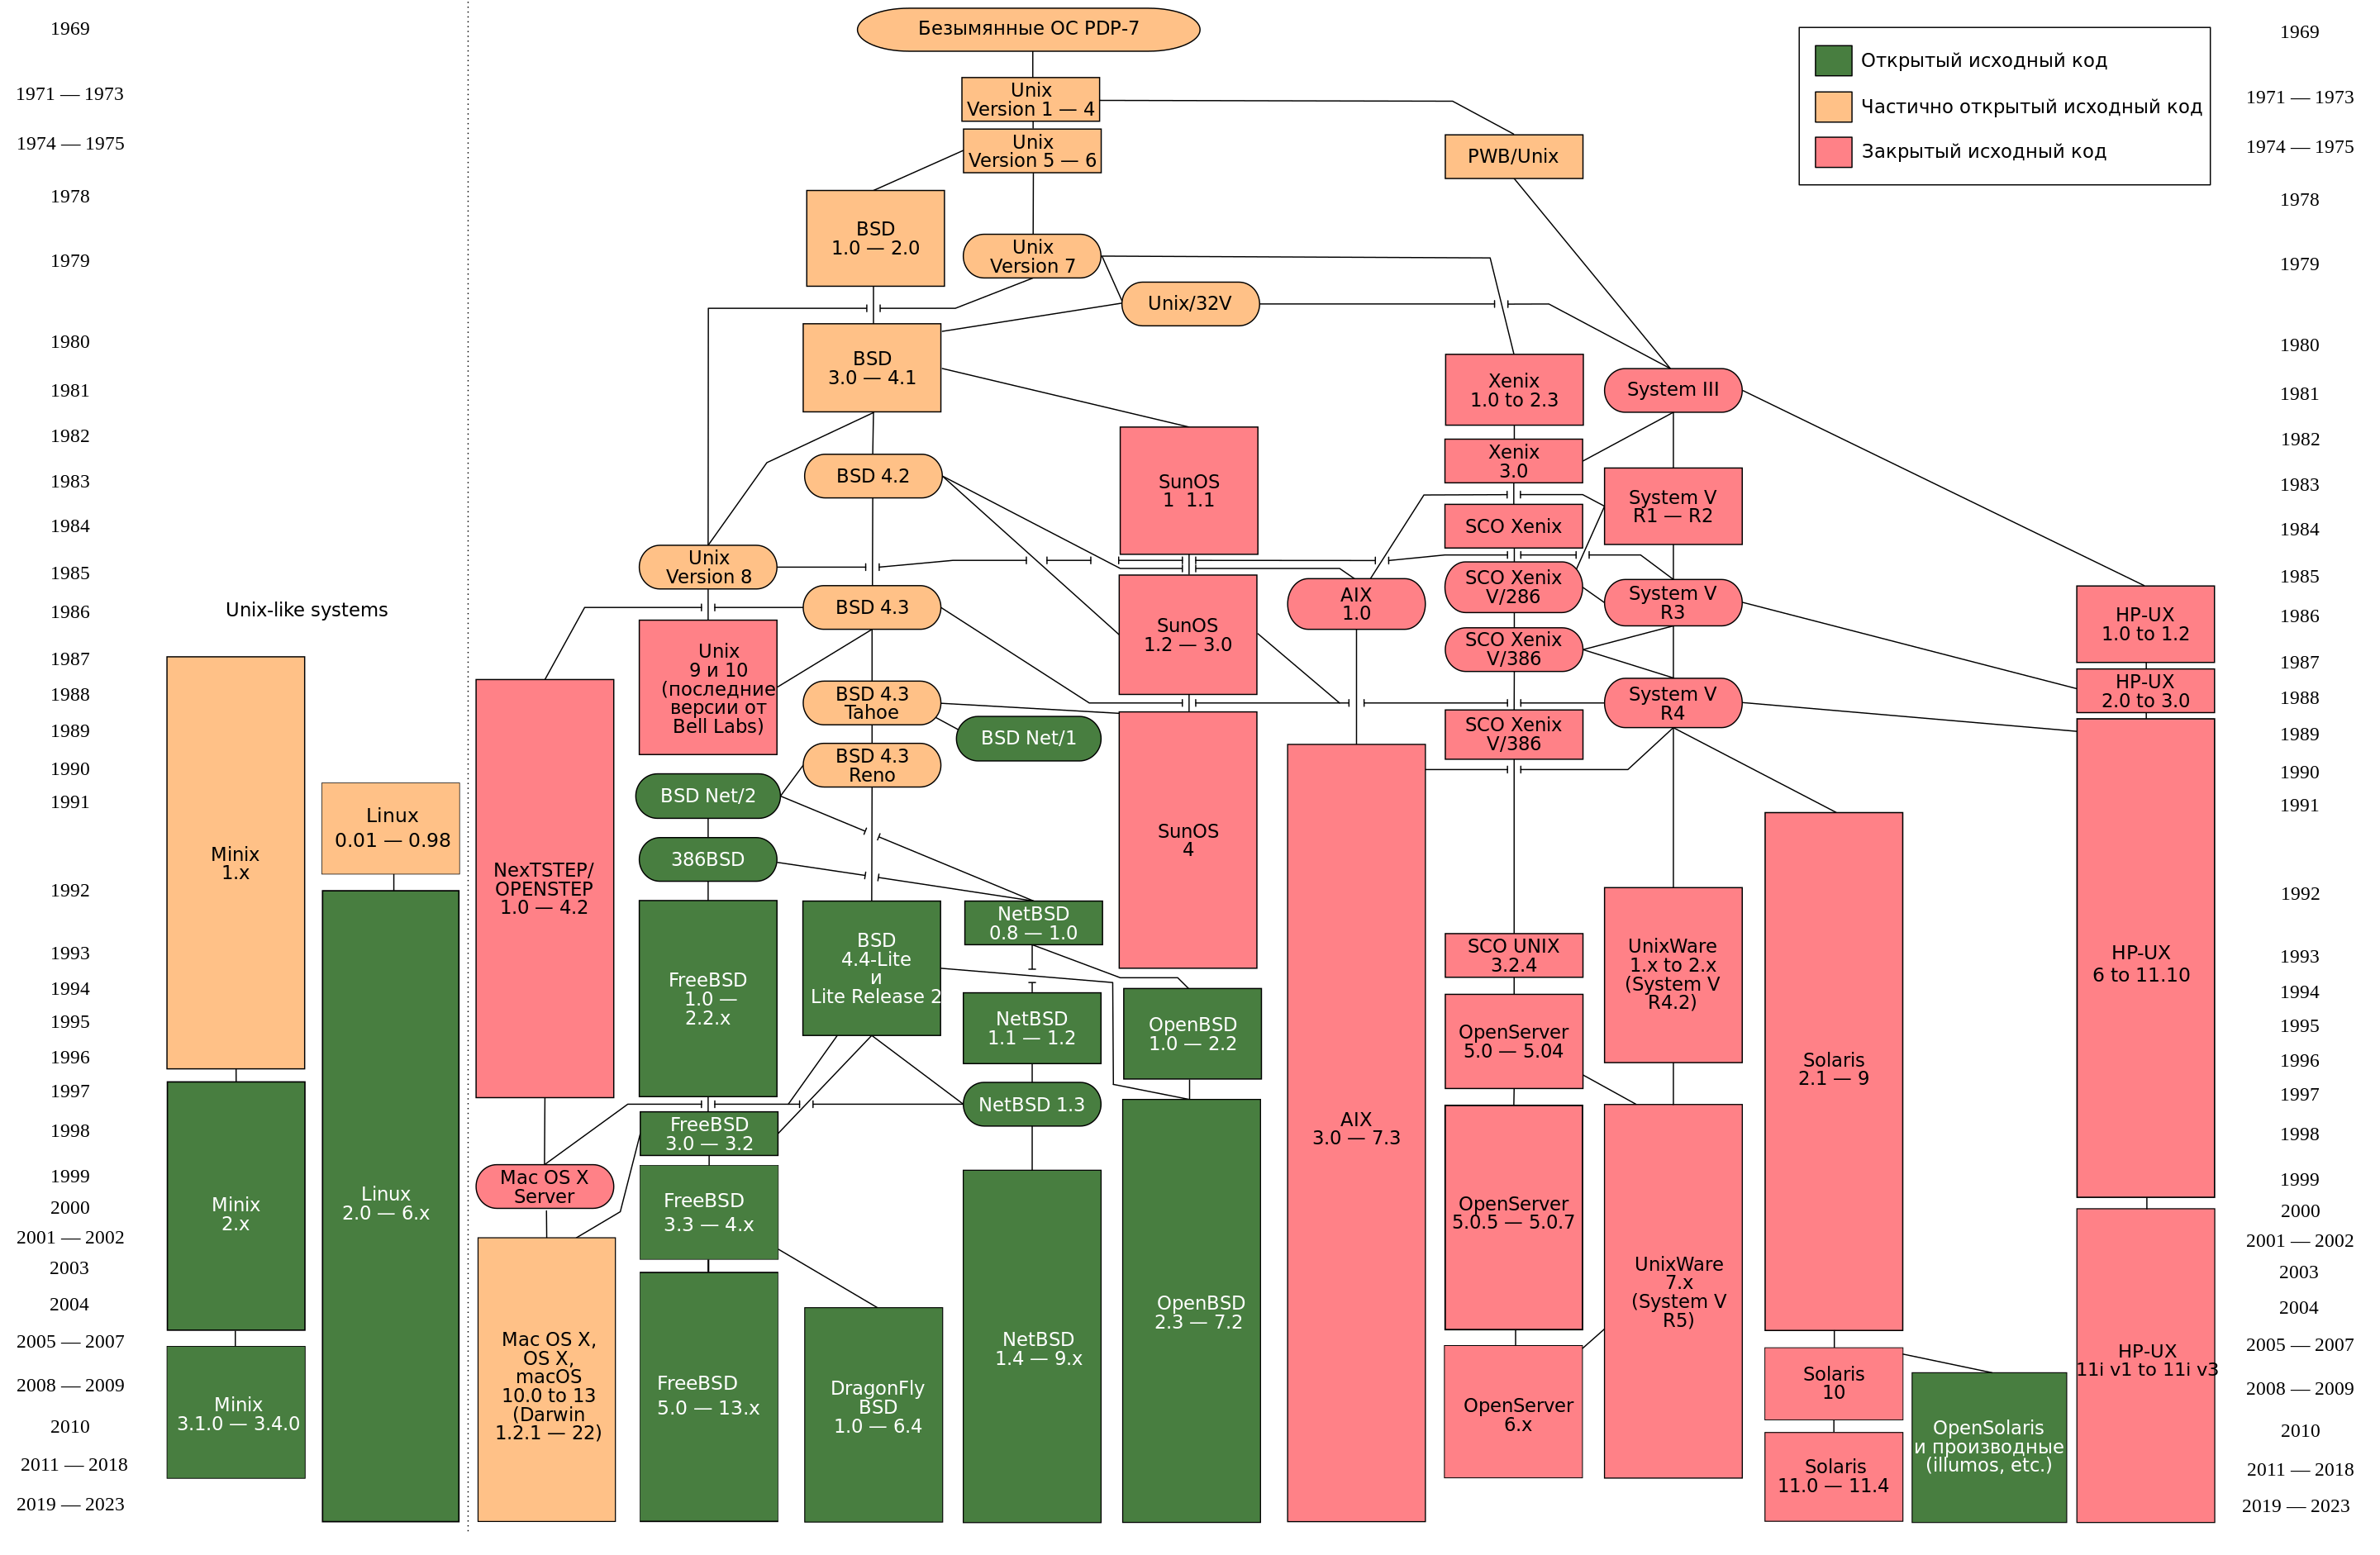
\includegraphics[width=0.9\textwidth]{unixHistory.png}
\end{center}

\subsection{Отличия от Windows}

Тут обсудим отличия Linux от Windows с точки зрения пользователя.
Вообще, это совершенно разные операционные системы, с разной философией, архитектурой и, конечно, пользовательским опытом, однако общего у них тоже довольно много (что неудивительно, похожие задачи всегда влекут похожие решения).
Вот с чем пользователь Windows, который впервые пересаживается на Linux, обязательно столкнётся.

\begin{itemize}
    \item Пакетный менеджер.
        В Linux приложения не скачиваются с непонятных сайтов, как принято в Windows, а ставятся из централизованных репозиториев с помощью установочных пакетов и специальной программы --- того самого пакетного менеджера.
        Причём, если в Windows программы обычно ставятся в Program Files и иногда имеют свою подпапку в папке пользователя, то в Linux приложение оказывается \enquote{размазанным} по файловой системе по определённым правилам, о которых чуть дальше.
        Поэтому установка, удаление, обновление и т.п. делается через пакетный менеджер, просто удалять программу с диска нельзя, и не принято встраивать в программы функциональность автообновления (например, VS Code обновляет себя под Windows, но обновляется силами пакетного менеджера под Linux).
        Пакеты могут зависеть друг от друга, поэтому прикладные программы, как правило, имеют в разы меньшие размеры, чем в Windows --- всё нужное уже, скорее всего, установлено в системе, и если нет, то поставится автоматически и может быть переиспользовано ещё кем-то.
        Пакетная система дистрибуции программного обеспечения уже наверняка знакома --- в Windows есть свой пакетный менеджер Chocolatey (но поскольку он не встроен в систему, о нём мало кто знает), есть Microsoft Store (но там своя атмосфера), ещё есть Android и iOS, где репозиторий централизованный и контролируется производителем.
        В Linux репозиторий обычно привязан к дистрибутиву и один, но никто не мешает добавить сколько угодно дополнительных, и тут это валидная модель распространения программы --- например, VS Code предоставляет репозиторий, где лежат пакеты самого VS Code и зависимостей.
        Скачивать программы с непонятных сайтов тоже можно, тем более что непонятные сайты обычно предлагают удобный способ установки под Linux (например, .NET ставится именно так, скриптом dotnet-install.sh с сайта Microsoft), но делается это только в случае, если в репозитории дистрибутива нужного пакета нет.
    \item Файловая система различает регистры в именах файлов и директорий, так что header.h и Header.h --- совершенно разные файлы.
        Поэтому на всякий случай всё обычно именуется со строчной через подчёркивание или дефис.
        Бывают, конечно, исключения (в дистрибутиве, на котором верстался этот конспект, например, есть директория \enquote{Рабочий стол}).
        У файлов нет атрибута \enquote{скрытый}, поэтому по соглашению скрытые файлы именуются с точки в начале.
        Кстати, все имена файлов --- в UTF-8.
    \item В файловой системе нет понятия \enquote{диск}, дерево файлов и директорий имеет один корень, директорию \enquote{/}.
        Абсолютно всё, включая файлы на разных физических дисках, флешках и сетевых шарах, лежит где-то в поддиректориях \enquote{/}.
        Есть понятие \enquote{монтирование} --- \enquote{прививание} внешней файловой системы внутрь какой-то из директорий \enquote{/}.
        Например, флешка может быть доступна по пути \enquote{/media/user/флешка/}.
        Монтирование можно выполнять вручную, но в подавляющем большинстве случаев оно выполняется само.
    \begin{itemize}
        \item Обратите внимание, слеши в Linux всегда прямые. 
            Windows умеет и так и так. но предпочитает обратные, Linux считает обратный слеш началом escape-последовательности.
    \end{itemize}
    \item Оконный менеджер не является частью операционной системы.
        В Windows управление окошками --- часть функциональности ядра, поэтому поменять их внешний вид и, тем более, функциональность, весьма сложно.
        В Linux есть как отдельные приложения низкоуровневые рисовалки, которые умеют рисовать собственно окна и обрабатывать события пользовательского ввода, так называемые \enquote{окноводы}, которые управляют размерами и размещением окон, и \enquote{среды рабочего стола}, которые добавляют всякие кнопки, панельки, виджеты, эффекты и т.п.
        И это более-менее ортогональные вещи, и по каждому пункту есть выбор, иногда весьма значительный.
        Поскольку всё это весьма конфигурируемо, каждый дистрибутив выглядит по-своему, да ещё и можно настроить под себя практически всё, вплоть до полной смены оконной подсистемы (что не так просто, но возможно).
    \item В Windows можно было набрать что-нибудь вроде \enquote{run.exe}, и если run.exe есть в текущей папке, он запустится.
        Linux скажет, что файл не найден, и начинающие пользователи могут быть шокированы, потому что вот же он лежит.
        Дело в том, что Linux не ищет по умолчанию запускаемые файлы в текущей директории, а сразу идёт смотреть пути из PATH --- по соображениям безопасности, чтобы нельзя было подложить что-то странное в директорию с программой.
        Чтобы запустить что-то из текущей директории, добавьте явную на неё ссылку: \enquote{./run.exe}.
        Ещё у файлов (и директорий) есть атрибут \enquote{исполнимый}, если атрибут не выставлен, запустить программу/скрипт не выйдет даже с точкой.
        Windows понимала, что файл исполнимый, по расширению, Linux тут на расширения не смотрит.
        Выставить атрибут \enquote{исполнимый} можно командой \mintinline{text}{chmod +x имя-файла}.
    \item В Windows большая часть системных настроек была в реестре, который по сути большая иерархическая база данных, которую без regedit.exe даже открыть-то не получится, причём и с regedit.exe там весьма сложно что-то содержательно редактировать и надо либо знать, что делаешь, либо пользоваться программами для настройки.
        В Linux есть правило, что все настройки должны быть человекочитаемыми и человекоредактируемыми.
        Поэтому обычно для конфигурации всего, даже самых дебрей ОС, используются простые текстовые файлы.
        При этом если опций много и файл большой, применяется соглашение с разделением такого конфига на несколько файлов и выкладыванием их в директорию <имя конфига>.d, где файлы перенумерованы в порядке их применения.
        Так что конфиги не только человекочитаемы, но ещё и обозримы и понятны (как правило).
    \item Очень важное различие --- папки в Linux называются директориями.
\end{itemize}

\section{Что бывает в мире Linux}

\subsection{Дистрибутивы}

Дистрибутив --- это готовое к установке ядро Linux, набор программ и пакетная экосистема, включающая в себя репозиторий (репозитории) пакетов, политику их включения в репозиторий и обновления, документацию и техническую поддержку.
В принципе, Linux можно собрать на коленке самостоятельно, без всяких дистрибутивов, но это достаточно большая работа, чтобы компании типа Canonical или Red Hat могли неплохо зарабатывать на распространении готовых дистрибутивов.
Почему --- в типичном Linux может быть больше десятка тысяч системных и прикладных программ, библиотек и технологий, и задача дистрибутива --- сделать так, чтобы они все вместе хорошо работали, что на самом деле весьма нетривиально.

Вот некоторые распространённые дистрибутивы --- так-то их сотни.

\begin{itemize}
    \item Ubuntu --- Linux для десктопных применений вместо Windows \enquote{по умолчанию}. 
        Большое сообщество, поддержка коммерческой компании, обновляется раз в полгода (в апреле и октябре).
    \item Mint --- дистрибутив на базе Ubuntu, предполагалось, что будет почаще обновляться, имеет свой менеджер рабочего стола, кому-то может быть приятнее, чем Ubuntu, но дело вкуса.
    \item Fedora --- старый проверенный дистрибутив от Red Hat и IBM (то есть за ним, как и за Ubuntu, коммерческие компании, которые его активно развивают), не любит проприетарное ПО (поэтому может быть не так удобен \enquote{вместо Windows}), но целостный, удобный и регулярно обновляемый. Достойный выбор.
    \item Debian --- ещё более старый и проверенный дистрибутив (первый выпуск в 1993 году, когда Linux ещё только появился), на его основе делалось большинство более модных и современных дистрибутивов (Ubuntu, Mint, даже SteamOS).
        Обновляется пореже.
    \item Arch --- дистрибутив на основе своего пакетного менеджера, в основе которого концепция частых (раз в месяц) обновлений.
        Для опытных пользователей.
    \item Gentoo --- дистрибутив, где всё надо собирать из исходников.
        Сейчас это на самом деле уже неправда, но философия дистрибутива была в том, чтобы вообще не распространять бинарные пакеты, а поставлять исходники и иметь на машине пользователя всё необходимое для сборки.
        Тогда пользователь может собрать ПО конкретно под своё оборудование конкретно так, как ему нужно.
        На современных машинах сборка под конкретную архитектуру позволяет добиться ускорения работы примерно на 1-2 процента, но ждать результатов компиляции несколько часов, так что сообщество сошлось на том, что того не стоит.
        Но любителям всё контролировать и настраивать под себя зайдёт (\emph{только} для опытных пользователей, не ставьте его как свой первый Linux!).
    \item Альт, РОСА, Астра, РЕД ОС --- самые известные российские дистрибутивы, как правило, платные с бесплатной версией.
        Альт и РОСА базируются на Mandriva (причём Альт отделился очень давно), Астра --- на Debian.
        Хороши тем, что сертифицированы для использования в том числе в государственных органах, и поэтому активно замещают Windows для рабочих нужд конечных пользователей.
        Бесплатные варианты не всегда хорошо поддерживаются, имеют довольно старые пакеты в репозиториях и местами содержат ошибки (TeX из репозитория на Альте у автора не заработал, какой-то файл положить забыли).
        Однако если хотите пережить отключение российского сегмента интернета, отзыв корневых сертификатов или прекращение обслуживания зоны .ru корневыми DNS-серверами, или просто не хотите, чтобы какой-нибудь драйвер принтера удалил вам все данные за то, что у вас ip-адрес из России, это вполне достойный выбор.
        Данный текст верстался на ROSA Fresh Desktop 2021.1 (хоть они и не платят за рекламу).
\end{itemize}

Вот картинка из википедии, которая перечисляет несколько больше дистрибутивов и показывает их взаимосвязь: \url{https://upload.wikimedia.org/wikipedia/commons/1/1b/Linux_Distribution_Timeline.svg} (дата обращения: 25.02.2024).
Обратите внимание, что это SVG, так что можно искать по названию дистрибутива.

\subsection{Пакеты}

Основой любого дистрибутива является пакетная система. 
Пакет --- это способ распространения приложений и библиотек в Linux, состоит из бинарников (собранных под какую-то целевую архитектуру), конфигурационных файлов, документации, иногда исходников%
\footnote{Большинство программ под Linux распространяется по традиции под лицензией GPL, которая требует распространения исходников --- однако не требует обязательно поставлять их прямо с бинарниками, поэтому часто пакет делится на собранную программу (или библиотеку или что угодно), которую обычно ставят пользователи, и отдельный пакет с исходниками, для тех, кто готов засучить рукава и что-то править. Иногда пакет просто приводит ссылку на репозиторий и на том успокаивается.}.
Также в пакете есть метаинформация --- как пакет называется, зачем он, версия (в формате semantic versioning --- мажорная и минорная версии, релиз; между минорными версиями гарантируется бинарная совместимость), зависимости (другие пакеты, которые должны быть установлены перед тем, как ставить этот).
Зависимости образую дерево, зачастую весьма ветвистое, потому что пакет в Linux --- это, как правило, не целое приложение, а что-то гораздо более мелкое, вплоть до конкретного конфигурационного файла.
Ещё бывают метапакеты --- пакеты, где есть \emph{только} зависимости.
Они нужны, чтобы сразу поставить пачку пакетов, нужных для решения какой-то общей задачи (например, сразу весь TeX).
Общий вид типичного имени пакета --- \mintinline{text}{<название>-<версия>-<выпуск>.<архитектура>} (где архитектура --- это подо что собран пакет, бывает noarch, то есть не важно, подо что, везде будет работать, или указание конкретной архитектуры процессора --- например, пакеты под i686 под arm не запустятся).

Пакеты хранятся в разных форматах.
Это всегда сжатая каким-то архиватором директория, так что скачанный пакет можно открыть и посмотреть обычным архиватором.
Детали в том, каким именно алгоритмом выполняется компрессия и как представляется метаинформация (и что в ней вообще есть --- например, \enquote{рекомендованные} пакеты).
Популярных форматов всего два --- .deb (из Debian, на базе которого делается много других дистрибутивов, например, Ubuntu) и .rpm (Red Hat Package Manager, Fedora и её многочисленные производные).
В общем, все дистрибутивы могут работать с пакетами всех форматов, но репозиторий дистрибутива всегда строится на чём-то одном, поэтому пакеты в другом формате будут несколько тяжелее в установке.
Это мягко говоря --- если у нужного пакета много зависимостей, можно замучиться их разрешать.

Для работы с пакетами есть утилиты, которые по уже готовому пакету могут его корректно поставить --- это не просто распаковать, а разложить по директориям, отметить в локальной базе пакетов, что такой-то установлен.
Для .deb это dpkg, для .rpm --- так и называется, rpm.
У них есть и графические оболочки.
Однако пользователь с ними напрямую обычно не взаимодействует, их вызывают пакетные менеджеры --- более высокоуровневые штуки, которые умеют укачать нужный пакет и его зависимости из репозитория, искать нужный пакет локально и в репозиториях дистрибутива и т.п.
Вот самые популярные пакетные менеджеры:

\begin{itemize}
    \item apt (Advanced Packaging Tool) --- используется в Debian и дистрибутивах на его базе: Ubuntu, Mint, Альт и т.п.
    \item yum (Yellowdog Updater, Modified) --- используется в старой Fedora и дистрибутивах на её основе.
    \item dnf (Dandified YUM) --- используется в новой Fedora и дистрибутивах на её основе, например, РОСА.
\end{itemize}

Функциональность пакетных менеджеров примерно одинакова (поскольку они одну задачу решают), но команды могут немного отличаться.

Также в Linux-сообществе набирает популярность подход с установкой приложения целиком со всеми зависимостями (к чему давно пришли в Windows), иногда даже с контейнеризацией.
Примеры менеджеров пакетов, реализующих такой подход --- Flatpak, Snappy, AppImage.
Они позволяют создавать пакеты, не зависящие от дистрибутива, что в традиционном подходе невозможно, и тем избавиться от dependency hell и необходимости для одного приложения поддерживать десяток пакетов для популярных дистрибутивов.
Недостаток --- значительно большие требования к дисковому пространству и интернет-каналу,, накладные расходы (хоть и не большие) по скорости работы на контейнеризацию.

\subsection{Среды рабочего стола}

Среды рабочего стола виднее всего пользователю, поэтому при выборе дистрибутива внезапно наиболее важный выбор, поскольку если UI неудобный, продуктивность работы даже с отличным прикладным ПО будет не очень.
Вообще, напомним, что в Linux графическая подсистема не является частью ядра, а обычно разделена на графический сервер и клиенты, которые, посылая запросы графическому серверу, рисуют окна и всё необходимое.
Графических сервера популярных два --- исторически первый X Server, более новый (ну как новый, 2008 года), но всё ещё не очень распространённый и не очень поддерживаемый Wayland.
Wayland считается более прогрессивным, но более болезненным для использования в ситуациях типа \enquote{пошарить окно в Teams} или даже \enquote{подключиться к проектору}.

Однако если всё хорошо, пользователь даже не знает, какой у него графический сервер.
Видит он среду рабочего стола.
Есть две известные среды:

\begin{itemize}
    \item GNOME и его производные (MATE, Cinnamon) --- используется в Ubuntu, Mint и много где ещё. Довольно легковесный и быстрый, но не очень конфигурируемый и без впечатляющих эффектов. Реализован на графической библиотеке GTK+.
    \item Plasma (ранее известный как KDE) --- используется по умолчанию в РОСА, в вариантах известных дистрибутивов --- например, KUbuntu (это буквально \enquote{Ubuntu на KDE}). Очень конфигурируемый и сложный в настройке, красивый, небыстрый (из-за кучи отключаемых графических эффектов), близок по UX оконной системе Windows.
\end{itemize}

Ещё бывает XFCE, совсем уж легковесная и нефункциональная оконная система, которую, однако, вполне можно поставить на какой-нибудь забытый сервер, чтобы не только из консоли работать, или на слабенький ноутбук (или слабенький одноплатник, который взрослую среду не потянет). 
Тоже на GTK+, так что в каком-то смысле младший брат GNOME.

Важно понимать, что среда рабочего стола образует некую экосистему приложений.
Есть приложения на GTK+, которые органично смотрятся в GNOME, но не очень хорошо интегрируются в Plasma и кажутся там противоестественными.
Есть приложения на Qt, которые везде смотрятся хорошо, но, возможно, у автора предвзятое мнение после нескольких лет опыта разработки на этой библиотеке.
Они, тем не менее, могут не выполнять принятые в GNOME соглашения, и потому не очень органично вписываться в привычный пользователям интерфейс.
Даже более важно то, что оконные приложения базируются на оконных библиотеках, которые базируются на низкоуровневых графических и вспомогательных библиотеках, так что:

\begin{itemize}
    \item поставить любое графическое приложение под любую среду рабочего стола вполне возможно, известные дистрибутивы имеют в репозиториях и Plasma (KDE), и GNOME, и всё, что нужно для их работы, но
    \item одно несчастное приложение, устанавливаемое на \enquote{неродную} среду, притянет в зависимостях большую часть среды, для которой оно было написано, что, скорее всего, ничего не сломает, но может быть совершенно негуманно по отношению к месту на диске и скорости скачивания.
\end{itemize}

\section{Файловая система}

Файловая система в Linux отличается от Windows довольно радикально, поэтому о ней следует поговорить отдельно и ещё до обсуждения консольных команд для работы с ней.

Файловая система --- суть набор inode (индексных дескрипторов) --- записей в файловой таблице, которые содержат метаинформацию о файлах (в частности, где на диске они физически лежат, права доступа).
В первых файловых системах inode-ы физически лежали в одном массиве в начале диска, и номер inode-а был его индексом в массиве (может, для большинства файловых систем и сейчас так, не знаю).
Важно то, что у каждого inode-а есть номер, его можно посмотреть командой \verb|ls -i|, и каждый inode --- это и есть файл, а всякие символьные имена файлов в директориях --- это просто ссылки на inode.
То есть можно понимать имя файла как указатель, а inode --- структуру данных в памяти, на которую указатель ссылается. 
Тогда будет неудивительна концепция жёсткой ссылки --- два файла в одной файловой системе, но в совершенно разных её местах, могут физически одним и тем же файлом.
Windows тоже так умеет, но про это никто не знает и никто не пользуется, тогда как в Linux такие вещи распространены.
Поскольку на один файл могут ссылаться несколько \enquote{имён файлов}, то удаление файла чем-то напоминает сборку мусора --- файл удаляется, только если на него не указывает больше никакая жёсткая ссылка.
Жестких ссылок на директории не бывает, потому что они другое, и физически на диске не лежат.

Бывают ещё символьные ссылки --- это прямой аналог ярлыков в Windows, файл, который ссылается на другой файл по пути до него (абсолютному или относительному).
Символьные ссылки используются гораздо чаще, чем жёсткие ссылки, потому что могут действовать через границы файловых систем (с диска можно ссылаться на директорию на флешке), могут ссылаться на директории и переживают копирование (если путь в ссылке относительный).
Для всех программ и утилит символьная ссылка --- файл или директория, на которую она ссылается.
Символьные ссылки, например, используются для разрешения альтернативных зависимостей, например, директория lib может быть символьной ссылкой на директорию lib32 или lib64, файл sh может быть ссылкой на оболочку командной строки bash, так что всем, кому не важно, какая именно оболочка нужна, могут просто sh вызывать.
И потом одной командой пользователь может перекинуть sh на zsh, и тем сменить оболочку.

У каждого файла есть режим доступа, кодирующийся тремя группами по три бита.
Три бита --- это Read, Write, Execute, почему трёхбитовых прав у каждого файла три --- потому что права выставляются отдельно для владельца, группы владельца и всех пользователей системы.
Кодируются права обычно трёхзначным числом в восьмеричной системе, например, 777 --- разрешено всё всем, или 700 --- владельцу можно всё, остальным ничего.
Чаще обозначаются буквами rwx, например, в выводе команды \verb|ls -l| может быть \verb|rw-r--r--| (владелец может писать и читать, остальные только читать).
Права можно поменять командой chmod (если у вас есть права на запись в файл), например, \verb|chmod +x имя-файла.txt| сделает его доступным для исполнения.
Без атрибута Execute запустить файл, даже если это скрипт или бинарник, нельзя --- специально, чтобы пользователь не запустил случайно какой-то файл, который ему прислали во вложении к письму с темой \enquote{Вы выиграли миллион!}.
Права у директорий тоже есть, но несколько менее интуитивны --- например, можно иметь права редактировать файлы в директории, если вы знаете имя файла, но одновременно с этим не иметь прав на просмотр списка файлов в этой же директории.

Ещё совершенно неожиданным для пользователей Windows может оказаться тот факт, что далеко не каждый файл в Linux лежит на диске.
Вообще философия Linux состоит в том, что всё, что поддерживает потоковый ввод-вывод --- файл.
Это позволяет использовать стандартные утилиты для работы с файлами для работы с такими штуками, а стандартных утилит много и они умеют очень многое.
Поэтому принято даже интерфейсы устройств, которые под Windows приходится программировать используя странные вызовы ядра, в Linux выводить в файловую систему, куда можно записать или прочитать строки определённого вида.

Простой пример --- файл \verb|/dev/null|, который содержит сразу символ EOF, и куда можно записать что угодно, и оно навеки исчезнет (этот факт часто используется, чтобы перенаправлять вывод гадящей на консоль программы).
Или \verb|/dev/random| --- писать туда можно с тем же эффектом, что и в \verb|/dev/null|, зато читать оттуда можно бесконечную последовательность \enquote{хороших} (то есть достаточно случайных, генерируемых посредством непрерывно накапливаемой системой энтропии, типа движений мышки) случайных чисел.
Есть даже директория \verb|/proc/|, где для каждого запущенного в системе процесса есть директория, где лежат файлы (ни в коем разе не на диске), из которых можно читать некоторую информацию о процессе или управлять им.
Так же в \verb|/proc/| есть и файлы с общей информацией о системе, например, \verb|/proc/cpuinfo|, их можно открыть блокнотиком (лучше просто напечатать командой cat).
Это настолько хорошо работает, что если вы делаете под Linux что-то такое, что долгое время запущено и может управляться извне или выдавать какую-то информацию/статус, это принято выводить как файл в файловой системе (например, датчики в роботе).

\subsection{Filesystem Hierarchy Standard}

Хорошая новость в том, что файловая система Linux и в целом всех Unix-подобных систем в целом стандартизована и многие директории там имеют стандартное назначение, узнав про которое можно будет довольно легко ориентироваться.
Стандарт называется FHS (Filesystem Hierarchy Standard), он уже лет 10 не обновлялся, поэтому не все дистрибутивы ему строго следуют, но в целом всё так.

Стандарт классифицирует файлы по двум независимым признакам --- изменяемые и статичные файлы, и разделяемые и неразделяемые.
Статичные файлы --- которые не меняются, если их не трогать (то есть при обновлении программы или изменении настроек --- сколько угодно, но для этого требуется некая воля администратора).
Разделяемые файлы --- это те, которые можно выставить в сеть и пользоваться ими с других машин (например, пользовательские данные).
Разные сорта файлов могут иметь разные настройки бэкапов, разные режимы доступа (например, статически файлы для обычного пользователя могут быть подмонтированы только для чтения), поэтому должны лежать в разных директориях.

Корневая файловая система, на которой находится директория \enquote{/} и образ ядра системы, содержит только самое необходимое для загрузки и восстановления системы в случае, если что-то сломалось настолько, что другие файловые системы уже не монтируются (например, утилиту mount, которая собственно за монтирование и отвечает).
Внутрь директории \enquote{/}, в её разные поддиректории, монтируются другие файловые системы.
Сделано так по историческим причинам, когда диски были маленькими, ну и чтобы было удобно работать на встроенных устройствах, где корневая система могла жить на отдельном очень маленьком, дешёвом и неэнергоёмком носителе, остальное монтировалось по необходимости.
Сейчас, однако, диски большие и дешёвые, поэтому нередко вообще вся система ставится на один раздел диска, и никто с монтированием и минимизацией стартового набора корневой файловой системы не заморачивается.
Поэтому современные дистрибутивы используют концепцию \enquote{joined root}, которая прямо нарушает стандарт FHS --- вовсе не отделять критичные для работы системы утилиты от всех остальных программ.

Всё не критичное для загрузки и аварийного администрирования системы лежит в директории \verb|/usr|.
Она по стандарту содержит в себе статичные файлы, поэтому может быть подключена в режиме \enquote{только для чтения}, никто не мешает иметь её на съёмном диске или вообще монтировать по сети.

Вообще, все поддиректории корня (директории \enquote{/}) фиксированы стандартом и авторам дистрибутивов и тем более разработчикам прикладных программ создавать дополнительные директории в \enquote{/} запрещено.
В Windows последних версий в целом тоже более-менее так, там запись в корень диска C требует административных прав, но это не останавливает инсталляторы (Python по умолчанию на полном серьёзе создаёт в корне по папке для \emph{каждой} своей версии), да и сама система имеет в корне файл подкачки и ещё какое-то барахло.
В Linux подкачка живёт на отдельном разделе, который даже никуда не монтируется, так что пользователь его и не увидит (справедливости ради, оперативная память сейчас тоже большая и дешёвая, так что подкачку часто отключают вовсе).

Стандартные директории в FHS таковы:

\begin{itemize}
    \item /bin --- нужные при запуске и поломке системы программы, которыми может пользоваться не только системный администратор, но и простые смертные, физически лежит в корневой файловой системе;
    \item /boot --- файлы загрузчика: конфигурация, часто образ ядра (образ на небольших системах может лежать в корне);
    \item /dev --- файлы устройств (это те самые \enquote{псевдофайлы}, которые не лежат на диске, и нужны для взаимодействия с устройствами);
    \item /etc --- локальная (то есть не разделяемая между машинами) конфигурация, например, тут находятся зарегистрированные в системе пользователи со своими паролями (в зашифрованном виде, конечно), конфигурация оконной системы;
    \item /lib --- библиотеки и модули ядра, разделяемые остальными программами и необходимые при старте системы;
    \item /media --- сюда монтируются внешние носители типа флешек;
    \item /mnt --- директория для временного монтирования, изначально пустая, но командой mount её содержимое заменяется на другую файловую систему; если хочется монтировать что-то постоянно, то уже в media (и настроив автоматическое монтирование в \verb|/etc/fstab|);
    \item /opt --- директория для дополнительных пакетов (обычно проприетарных);
    \item /sbin --- нужные при запуске и поломке системы программы, которыми предполагается что будет пользоваться системный администратор (и имеющие соответствующие права), \enquote{system binaries};
    \item /tmp --- временные файлы, создаваемые приложениями и системой в ходе работы, чистятся при каждой загрузке;
    \item /usr --- вторичная иерархия (примерно та же иерархия, но из некритичных файлов);
    \begin{itemize}
        \item сейчас популярен \enquote{joined root}, когда \verb|/bin| --- это символическая ссылка на \verb|/usr/bin|, а \verb|/sbin| --- на \verb|/usr/sbin|;
    \end{itemize}
    \item /var --- изменяемые данные, которые появляются по ходу работы приложений и системы --- прежде всего, всякие логи;
    \item /home --- директория для домашних директорий пользователей (то есть директорий, где хранятся всякие специфичные для пользователей файлы, типа локальной конфигурации или сохранений игр);
    \item /root --- как /home, но для администратора, а поскольку на аккаунте администратора не должно быть сохранений игр, обычно пустая или не создаётся вовсе;
    \item /lost+found --- результат деятельности fsck, inode-ы, которые есть на диске, но на которые не указывают никакие имена --- так может случиться при повреждении файловой системы, например, при выключении электричества прямо в процессе записи файла: fsck при следующей загрузки такие inode-ы найдёт и сложит в \verb|/lost+found|.
\end{itemize}

\section{Работа с консолью}

Теперь очень кратко рассмотрим основные знания про работу с консолью Linux, поскольку с консолью тут придётся взаимодействовать гораздо чаще, чем в Windows, и надо уметь использовать её эффективно.

\subsection{Основные команды}

Вот, пожалуй, самые частоиспользуемые команды в консоли Linux.

\begin{itemize}
    \item cd --- переход в директорию, так же, как в Windows; абсолютные пути начинаются с /, относительные без / в начале, могут содержать \enquote{.} или \enquote{..}, которые имеют тот же смысл, что и в Windows (текущая директория и родительская директория соответственно --- например, \verb|cd .| ничего не делает, \verb|cd dir/..| тоже).
    \item ls --- показать содержимое директории. 
        Без параметров --- текущей, с параметром --- по заданному пути. 
        Имеет много ключей, например, \verb|-a|, который заставляет ls показывать и скрытые файлы тоже, или \verb|-l|, который показывает файлы с правами доступа, размером, датой последней модификации и т.п.
    \item mkdir --- создать директорию, как в Windows.
        С ключом \verb|-p| создаёт весь переданный в качестве параметра путь, иначе --- только поддиректорию в текущей.
    \item touch --- обновить время последнего обращения к файлу или создать пустой файл.
        Наверное, самый простой способ создать файл в Linux.
        Ещё полезен в скриптах сборки, чтобы заставить систему сборки пересобрать файл, даже если не было изменений с последней сборки.
    \item echo --- распечатать что-то в консоль, как в Windows.
    \item cat --- вывести содержимое файла на консоль прямо как есть.
    \item cp --- скопировать файл или директорию, так же, как в Windows.
    \item mv --- переместить файл или директорию со всем содержимым.
    \item rm --- удалить файл или директорию. 
        Удаляет только один файл или директорию, если она пустая, что крайне неудобно, поэтому обычно используется с ключом \verb|-rf| (Recursive, Force) --- рекурсивно удалить всё поддерево, не спрашивать подтверждения.
        Если не знаете, что делаете, обычно плохая идея.
        Например, \verb|rm -rf *.txt| удалит все файлы .txt в текущей директории, а \verb|rm -rf * .txt| удалит всё вообще.
        Есть ещё старая шутка про \verb|rm -rf /|, но от обычного пользователя эту команду вряд ли дадут исполнить.
    \item ln --- создать ссылку на файл или директорию.
        Символьные ссылки создаются с ключом \verb|-s|, жёсткие ссылки ключа не требуют, но создаются только на файл.
    \item sudo --- запустить от имени суперпользователя.
        Например, \verb|sudo rm -rf /| таки убьёт вам систему.
        sudo приходится пользоваться довольно часто, потому что обычные пользователи в Linux не могут ничего, что влияет на всю систему (Linux сразу создавалась многопользовательской и сетевой, так что неудивительно).
        Даже установка пакета --- всегда с sudo.
        Хорошая новость в том, что если пользователь состоит в группе sudoers или wheel (а по умолчанию при установке системы в большинстве дистрибутивов первый пользователь туда добавляется), никаких паролей или чего-то вводить не надо, sudo просто молча исполняет команду.
        Тем не менее, sudo честно переключает пользователя, то есть в команде, исполняющейся из sudo, например, пользовательская домашняя директория будет \verb|/root|, а не \verb|/home/имя-пользователя|.
\end{itemize}

\subsection{Продвинутые возможности консоли}

Тут поговорим о том, что ещё может консоль, помимо исполнения команд.

Во-первых, есть вайлдкарты (wildcards), они же глобы (globs) --- шаблоны имён файлов или директорий.
В примере выше \verb|rm -rf *.txt| вот это \verb|*.txt| --- это вайлдкарт, сопоставляющийся каждому файлу с расширением .txt в текущей директории.
Вайлдкарты раскрываются \emph{до} вызова команды, если хоть один файл подходит под вайлдкарт, так что если в директории есть два файла 1.txt и 2.txt, то команда выше будет исполнена как \verb|rm -rf 1.txt 2.txt|. 
Если ни одного файла .txt нет, параметр передаётся в команду как есть, то есть rm увидит \verb|*.txt| на входе.
Вот ещё пара примеров синтаксиса вайлдкартов: \verb|file[1-8]| (файл, заканчивающийся на цифру от 1 до 8), \mintinline{text}{file*} (файл, имя которого начинается с file, а дальше неважно).
Символ \verb|?| соответствует одному любому символу (\verb|*| --- сколько угодно любых символов), символ \verb|!| внутри квадратных скобок означает \enquote{не} --- например, \verb|file[!a-z]| соответствует всем файлам, имя которых начинается с \verb|file|, но дальше не строчная буква.
И да, это те самые шаблоны, которые надо писать в .gitignore, чтобы git не пытался коммитить всякий мусор в репозиторий --- git создавался как набор консольных скриптов под Linux, в конце концов.

Во-вторых, есть переменные окружения и квотирование. Переменные окружения в Linux работают так же, как в Windows, разве что оператор подстановки --- это \verb|$|, а не \verb|% %|.
И пути в \verb|PATH| разделяются двоеточиями, а не точками с запятой.
Переменная выставляется обычной командой \verb|=|, например, \verb|PATH=$PATH:/home/user/.dotnet|, но это действует на одну строчку.
Чтобы новую переменную видели все запускающиеся из текущей консоли программы, надо воспользоваться командой \verb|export|, например, \verb|export PATH=$PATH:/home/user/.dotnet|, чтобы видели все консоли, вписать этот export в файл .bashrc в домашней директории (и перезапустить консоли), чтобы все пользователи --- в /etc/profile.

Квотирование --- это заключение строки в кавычки.
Сильное квотирование --- это одинарные кавычки, внутри них текст интерпретируется шеллом и передаётся в команду как есть, например, \verb|echo '$PATH'| выведет на экран \verb|$PATH|.
Внутри одинарных скобок вайлдкарты не раскрываются и подстановка переменных окружения не выполняется.
Слабое квотирование --- это двойные кавычки, внутри них выполняется подстановка, но не раскрываются вайлдкарты.
Так что \verb|echo "$PATH"| выведет таки текущее содержимое \verb|PATH|, но \verb|echo "*.tex"| выведет \verb|*.tex|, даже если в директории есть теховские файлы.
Кстати, \verb|echo *| в силу правил раскрытия вайлдкартов работает как \verb|ls| (и да, не выведет скрытые файлы).

Вот ещё четыре полезные команды, которые помогают найти файл или нужную команду.

\begin{itemize}
    \item which --- найти программу в путях из PATH (так можно узнать, что именно запустится, когда мы наберём имя команды).
    \item whereis --- вывести все места, где находится нужная программа (например, если .NET SDK после ряда неудачных попыток его правильно поставить оказался в трёх разных директориях, она их покажет).
    \item find --- найти файл, по имени, содержимому и много чему ещё: например, \verb|find /usr/share/doc -name README| найдёт все файлы с именем \verb|README| в \verb|/usr/share/doc|. 
        Имеет ключ \verb|-exec|, где можно написать команду, которую надо выполнить с каждым файлом (то есть, например, \verb|find . -name "*.csproj" -exec "dotnet build {} \;"| сами догадайтесь, что сделает).
        Вообще, find имеет много полезных ключей, возможность комбинировать условия поиска и чего только не делать.
    \item locate --- ищет по именам, но не только в именах файлов, но и в путях.
        Например, \verb|locate /usr/share/*/README|.
\end{itemize}

\subsection{Управление процессами}

Консоль вообще нужна прежде всего для управления программами, а запущенная программа в операционной системе называется \enquote{процесс}. 
Первое, что надо уметь делать с процессами --- это их останавливать, это делается, как и в Windows, сочетанием клавиш Ctrl-C.
Например, \verb|cat /dev/random| может поставить вас в неловкую ситуацию, выйти из которой можно, как раз нажав Ctrl-C.
На самом деле, Ctrl-C посылает сигнал процессу --- команду в его очередь сообщений (как и в Windows), конкретно Ctrl-C шлёт процессу SIGINT.
Поэтому, кстати, скопировать текст из консоли надо не Ctrl-C, а Shift-Ctrl-C.

Ещё бывает Ctrl-Z, он шлёт текущему процессу сигнал SIGTSTP --- Temporary Stop, поставить процесс на паузу.
Его можно будет перезапустить командой \verb|fg| (от \enquote{foreground}) или отправить работать в фоне командой \verb|bg| (от \enquote{background}).
В фоне процесс будет делать своё дело, выводить на консоль, если вывод не перенаправлен, но в консоль в это время можно вводить новые команды.
Можно прямо при запуске указать процессу запускаться в фоне, оператором \verb|&|, например, \verb|okular 06-intro-to-linux-text.pdf &|.

Есть отдельные команды kill и killall, которые, несмотря на агрессивное название, посылают указанному процессу (процессам) сигнал.
Например, \verb|killall -2 okular| отправит сигнал SIGINT всем процессам с именем okular, так, будто вы нажали Ctrl-C каждому (даже если они были запущены не из консоли, так что жать Ctrl-C негде).
SIGINT, однако, процесс может проигнорировать (почему, вы думаете, bash не закрывается, если вы случайно Ctrl-C нажали).
Более надёжно послать процессу сигнал SIGKILL (\verb|killall -9|), его игнорировать нельзя (это скорее сигнал операционной системе, что всё).
kill отличается от killall тем, что принимает идентификатор конкретного процесса (pid, от process identifier).
Полезно, когда вы хотите убить не все экземпляры программы N, а только один, который вышел из-под контроля.
Напомним, что kill/killall позволяют слать любые сигналы, не только SIGKILL.

Чтобы узнать pid процесса, можно посмотреть список процессов, запущенных в ОС.
Может, вы помните из текста выше, что можно глянуть содержимое директории \verb|/proc| и вручную разобраться, кто там кто, но гораздо проще использовать команду \verb|ps|.
Без параметров она показывает список процессов текущего пользователя, запущенных из текущего шелла, что обычно не очень интересно.
\verb|ps -e| покажет все процессы в системе, но их может быть многовато, чтобы это было полезно.
Есть команда \verb|top|, которая показывает самые ресурсоёмкие процессы в системе, обновляя данные по ним в реальном времени.
Выход --- клавишей \verb|q|.

Ещё одна очень важная возможность консоли --- перенаправление ввода-вывода.
Оператор перенаправления \verb|>| перенаправляет вывод в файл, например, \verb|echo "Hello, world!" > out.txt| создаст файл \verb|out.txt| со строкой \verb|Hello, world!| внутри.
Есть в каком-то смысле парная команда \verb|>>|, она не перезаписывает файл целиком, а добавляет вывод в конец.
Однако самая интересная команда перенаправления в Linux --- это пайп: \verb/|/.
Она перенаправляет стандартный вывод одного процесса на стандартный вход другого, так что, например, \verb/echo lol | wc/ выведет результат стандартной программы wc (word count) на строке \enquote{lol}.
Из пайпов можно собирать целые конвейеры обработки, например, \verb/cat file.txt | sort | uniq | wc -l/ возьмёт содержимое файла file.txt, отсортирует строки в нём в лексикографическом порядке, удалит повторяющиеся и посчитает, сколько строк осталось.
Это, собственно, и есть Linux way --- иметь в системе кучу мелких программок и удобный шелл с пайпами, который позволяет собирать сколь угодно сложные сценарии обработки данных прямо в консоли.
Вообще, любой нормальный шелл в Linux --- это полноценный язык программирования (хоть и такой себе в плане современной языковой науки, но, например, рисование .png-шек псевдографикой чисто на шелле --- это домашка первого курса некоторых вузов).
Мы тут не будем углубляться в детали, но если кому интересно, есть куча документации, и это всё равно будет крайне полезно, если планируете свою карьеру в любом embedded или DevOps.

\subsection{Команды для работы с текстом}

Есть набор команд для чтения и обработки текстовых файлов, которые крайне полезны, поскольку в Linux все настройки --- это текстовые файлы, логи системы и программ --- текстовые файлы, даже устройства и метрики работы системы --- текстовые файлы.
Некоторые команды мы уже видели выше:

\begin{itemize}
    \item sort --- отсортировать файл в том или ином порядке, умеет сортировать лексикографически, по датам и версиям, с разными другими настройками;
    \item uniq --- работает только для отсортированных файлов (или входного потока, перенаправленного из sort), убирает повторения;
    \item wc --- считает количество символов, слов и строк.
\end{itemize}

\begin{itemize}
    \item head, tail --- как cat, только вывести первые n строк из файла (по умолчанию 10).
        \verb|tail -f| выводит последние n строк файла непрерывно, так можно наблюдать за обновляющимися логами.
    \item more, less --- интерактивные читалки, less более новая и умеет скроллить файл вперёд-назад (поддерживая Page Up/Page Down).
        Выход по клавише q, как обычно.
        Есть ещё most, но ни разу не пользовался.
    \item sed, awk --- потоковые текстовые редакторы, как бы странно это ни звучало.
        Умеют найти и заменить шаблон (обычно регулярное выражение), при этом awk считается более продвинутым, но sed более удобным для командной строки и скриптов.
        Не то чтобы часто приходится пользоваться, но sed позволяет прямо из коробки в одну строчку писать скрипты, которые на Windows потребовали бы Python или чего-то такого.
        Считается приличным знать и уметь любому опытному пользователю Linux.
    \item vim --- полноценный интерактивный текстовый редактор в консоли.
        Очень старый, так что совершенно не уважает привычный интерфейс пользовательских редакторов, но достаточно удобный, чтобы многие его использовали как основной редактор и даже полноценную IDE, поскольку он очень хорошо интегрирован в консоль и имеет развитую систему плагинов.
        Обязательно хотя бы базовое редактирование на нём освоить, потому что если вдруг графическая оболочка с любимым VS Code или чем-то таким недоступна, то vim и его аналоги могут быть единственным способом редактировать конфиги, которые позволят эту самую графическую оболочку починить (ну или по ssh удалённо работать на сервере, где графической подсистемы нет вообще, потому что незачем).
        У него два режима --- в котором он пищит в в котором всё портит, переключение --- клавишей \enquote{i} и \enquote{Esc}.
        Выход --- из режима, когда он пищит, клавишами \enquote{:}, затем \enquote{wq} (или \enquote{!q}, если без сохранения).
\end{itemize}

\subsection{Ещё полезные штуки консоли}

Вот список случайных фактов о линуксовой консоли, которые могут понадобиться:

\begin{itemize}
    \item Табуляция --- ваш лучший друг.
        Она автодополняет текущую команду, причём контекстно. 
        Например, если вы пытаетесь открыть .pdf-файл командой okular, пишете \enquote{ok}, жмёте Tab, оно дополняется до okular, жмёте Tab ещё раз --- оно выводит список всего, что okular может открыть (и поддиректорий), начинаете вводить нужную, жмёте Tab, оно дописывает.
        Экономит кучу времени.
    \item .bashrc --- скрипт, который исполняется каждый раз, когда вы запускаете bash вручную.
        .bash\_profile --- скрипт, запускающийся при логине в систему с помощью bash.
        Оба лежат в домашней директории пользователя, оба скрытые (что понятно, потому что они начинаются с точки).
        Туда можно писать что угодно на языке шелла, но особенно полезна команда \verb|alias|, которая позволяет задать синоним для произвольной строки и использовать её как команду.
        Например, \verb|alias gcc="gcc -lm -g -Wall -Wextra"| автор использует для компилирования домашки по Си, вызывая просто gcc и получая сразу линковку с математической библиотекой, отладочную информацию (на случай, если надо будет потыкать программу консольным отладчиком gdb) и все разумные предупреждения.
    \item Кстати, вайлдкарт \verb|~| раскрывается в домашнюю директорию текущего пользователя, так что \verb|cat ~\.bashrc| позволит вам посмотреть на свой .bashrc из любого места файловой системы.
    \item Midnight Commander --- консольный файловый менеджер наподобие far под Windows (но несколько менее функциональный и удобный).
    \item reverse-i-search --- поиск по истории вводимых в консоли команд.
        Так-то историю команд можно скроллить стрелками \enquote{вверх}/\enquote{вниз}, что очень удобно, чтобы не вводить похожие команды дважды.
        Но если нужная команда вводилась когда-то давно, можно нажать Ctrl-R и начать её вводить, консоль её найдёт и по нажатию Esc или стрелки \enquote{вправо} оставит в командной строке для редактирования.
        Ctrl-S прокручивает историю команд вперёд, но есть нюанс (\url{https://stackoverflow.com/questions/17760474/reverse-intelligent-search-reverse-i-search-how-to-get-previous-result?rq=1} (дата обращения: 26.02.2024)).
    \item Ctrl-W удаляет слово под курсором (влево до пробела), Ctrl-U --- до начала строки, Ctrl-K наоборот, до конца строки.
        Ctrl-стрелки \enquote{влево}/\enquote{вправо} позволяют прыгать по словам (в отличие от Ctrl-W считают разделителем и \enquote{-} и т.п.).
        Ctrl-A и Ctrl-E --- ставят курсор в начало или конец строки.
    \item Любой текст в консоли можно выделить мышью, потом просто кликнуть средней кнопкой мыши в нужном месте --- и он вставится (не только в консоли это работает).
        И это делается \emph{не} через буфер обмена, так что информация в буфере обмена при этом не стирается.
        Сравните это с адом, через который надо пройти, чтобы в Windows что-то копировать из консоли, особенно если это не PowerShell.
    \item Для ввода специальных символов (типа тире) используется клавиша Compose.
        Она по умолчанию может быть не настроена вовсе, но можно поковыряться в настройках своей оболочки рабочего стола и повесить её на какую-нибудь не очень нужную клавишу, типа правого Ctrl (хотя тут такое, он удобно расположен близко к стрелкам, а Ctrl-стрелки часто нужны).
        Дальше жмём Compose, жмём трижды на минус --- получаем тире.
    \item Ctrl-Alt-F1, Ctrl-Alt-F2 и т.д. позволяют переключаться (прямо на рабочей системе) между графической подсистемой и чисто текстовым терминалом.
        Нужно, \sout{если} когда графическая подсистема помрёт из-за ошибки в конфигурировании и надо будет её оживлять из консоли.
        Текстовые терминалы работают всегда, в чём их важнейшее преимущество.
        Ctrl-Alt-Backspace (дважды) позволяет перезапустить графический сервер и все процессы, им порождённые, без перезапуска всей ОС.
    \item Всегда имеет смысл ставить проприетарные драйвера для видеокарты, и они почти никогда не ставятся по умолчанию.
        Как именно ставить, может зависеть от дистрибутива --- в паре российских дистрибутивов, которыми автор пользовался, для этого была целая специальная программа, которую можно было запустить (из консоли), и она сама ставила нужные драйвера nvidia.
        Linux по политическим мотивам не включает по умолчанию проприетарное ПО, потому что видение сообщества в том, что ПО должно быть свободным и поставляться только вместе с исходниками, а жадные корпорации, которые не хотят раскрывать свои исходники, могут идти под Windows.
        Но пока коммунизм не наступил, приходится ставить проприетарные драйвера видеокарты, принтера (скорее всего, хотя в Linux очень крутая система управления печатью cups, которая может и сама справиться, но если вдруг нужен ещё и сканер...), и даже кодек для MP3-файлов, если они нужны.
\end{itemize}

\section{Где брать документацию}

В Linux, в отличие от Windows, к документации по традиции относятся очень серьёзно.
Документация стандартизована, включена как составная часть во многие пакеты (можно сказать, в почти все, если автор не выделил сознательно пакет с документацией отдельно в силу огромного её объёма), хорошо поддерживается, есть системные утилиты для поиска и просмотра, которые, конечно, прекрасно работают в консоли.

Первая такая утилита --- \verb|man| (от слова \enquote{manual}).
Это та самая man, к которой отсылает знаменитое восклицание \enquote{RTFM} --- краткая документация, доступная для всех стандартных утилит Linux, многих файлов конфигурации, форматов и т.п.
Состоит из девяти тематических разделов, где первый --- это пользовательские программы, второй --- системные вызовы и т.д.
Так что одна и та же штука может встречаться в нескольких разделах сразу, если доступна, например, и как консольная команда, и как функция API системы.
И поэтому при ссылке на man-документацию обязательно указывают раздел, например, \verb|man top| выведет \verb|top(1)| --- пользовательская программа.
man открывает документацию в системном \emph{пейджере}, обычно это less (так что выход по q, как обычно).

Команда whatis --- типа оглавления man-документации, выводит однострочную справку по каждой man-странице, найденной по указанной строке.
Например, \verb|whatis top| выдаст \verb|top (1)              - display Linux processes|.

Команда apropos позволяет искать по man-документации, не только в заголовках, но и по телу справки.
Например, \verb|apropos top| выдаст кучу всего, потому что строка запроса коротковата.

Второй формат справки --- info-страницы и команда info для их просмотра.
Формат info считается более прогрессивным, в частности, поддерживает гиперссылки (в консоли прямо).
Одно может вроде как генериться из другого, так что для основных системных утилит есть и info-страницы, можно смотреть их.

Ещё очень важный источник документации --- документация вашего дистрибутива.
Она как повезёт, бывает хорошей, бывает так себе, бывает просто набором бессвязных статей на вики и постов на форуме (напомним, что в Linux-сообществе никто никому ничего не должен).
Тем не менее, очень многие вопросы специфичны для дистрибутива, и никакие man-ы тут не помогут.

Ещё есть списки рассылки по электронной почте, настоящие линуксоиды по традиции используют их, но как-то прошлый век.

\end{document}
